\documentclass[conference]{IEEEtran}
\usepackage{graphicx}
\usepackage{amsmath}
\usepackage{amssymb}
\usepackage{booktabs}
\usepackage{hyperref}
\usepackage{subcaption}
\usepackage[utf8]{inputenc}

\title{Diffusion-Based Map Completion for\\Frontier Exploration}
\author{
\IEEEauthorblockN{Moin Mattar}
\IEEEauthorblockA{Department of Computer Science\\
Dartmouth College\\
Hanover, NH 03755\\
moin.a.mattar.28@dartmouth.edu}
}

\begin{document}
\maketitle

\begin{abstract}
We present a conditional denoising diffusion model for occupancy grid completion that enables smarter frontier-based exploration. Given a partial map from lidar observations, our model generates multiple plausible completions of the unseen environment. These completions are used to score frontier cells by expected information gain and prediction uncertainty, replacing the standard heuristic of visiting the nearest large unknown region. Trained on 2.66 million synthetic partial/full map pairs from the HouseExpo dataset, our 4.2M-parameter U-Net achieves 82\% pixel accuracy and 0.62 IoU on single-scan inputs, improving to 0.88 IoU with realistic multi-scan coverage. In offline frontier scoring evaluation, our approach selects frontiers with 24.5\% higher actual information gain compared to the heuristic baseline, with the diffusion scorer winning or tying on all 10 test maps.
\end{abstract}

\section{Introduction}

Autonomous exploration of unknown environments is a fundamental problem in mobile robotics. The standard approach, frontier-based exploration~\cite{yamauchi1997frontier}, identifies cells on the boundary between known and unknown space and drives the robot toward them. While effective, na\"ive frontier selection uses simple heuristics such as nearest-frontier or largest-frontier, ignoring the structural priors inherent in built environments: walls tend to continue, rooms have regular shapes, and hallways connect spaces.

Recent work has applied learned models to predict unseen map regions from partial observations~\cite{shrestha2019learned}. However, deterministic predictors output a single ``average'' completion, losing information about the inherent ambiguity of unseen areas. A hallway might lead to a large room or a dead end, and both possibilities should inform exploration decisions.

We propose using a conditional denoising diffusion probabilistic model (DDPM)~\cite{ho2020ddpm} to generate \textit{multiple} plausible map completions from a partial occupancy grid. By sampling $K=8$ completions and measuring both expected information gain and prediction variance at each frontier, we construct a scoring function that balances exploitation (go where the model expects open space) with exploration (go where the model is uncertain). This approach directly connects to the uncertainty-seeking behavior studied in information-theoretic exploration~\cite{bourgault2002information}.

\begin{figure*}[t]
\centering
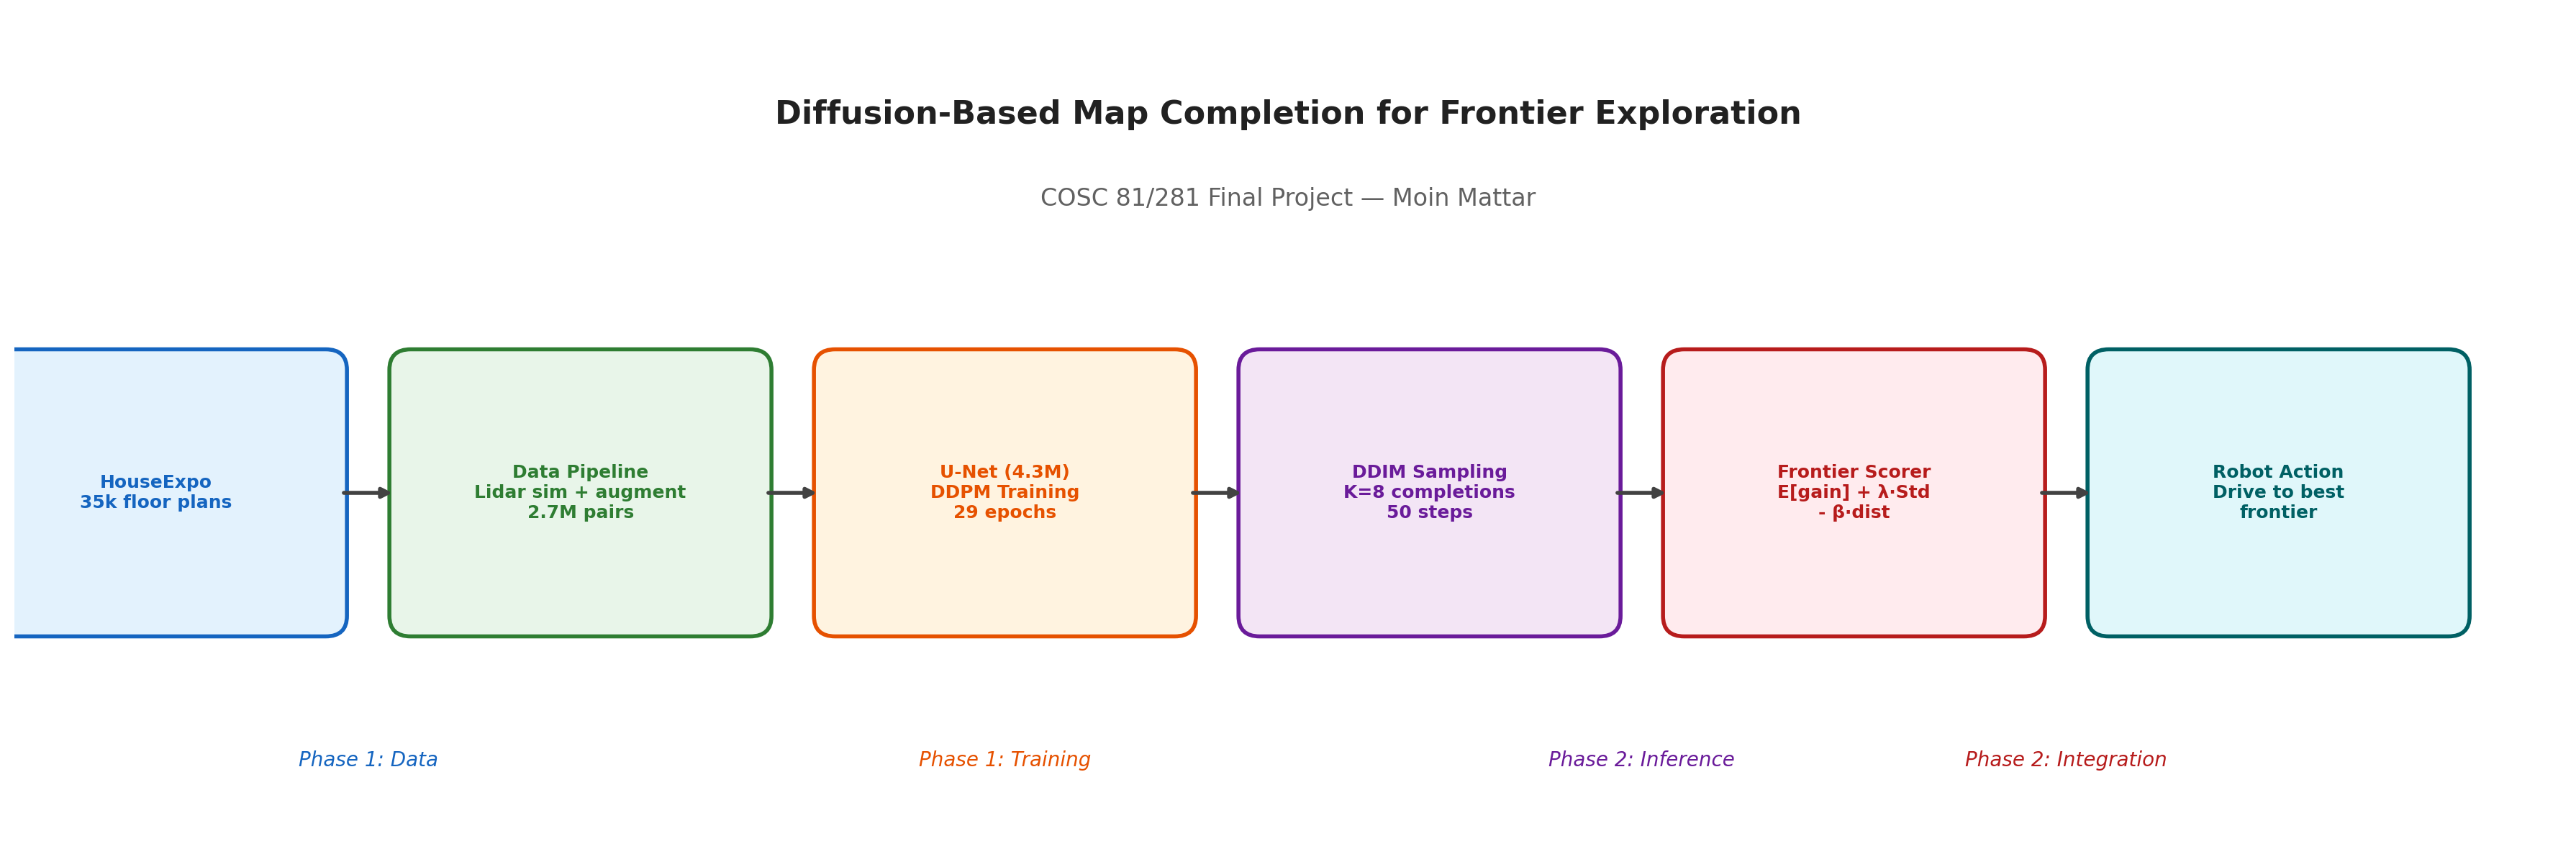
\includegraphics[width=\textwidth]{fig_pipeline.png}
\caption{System pipeline: HouseExpo floor plans are used to generate training data via lidar simulation. The trained U-Net performs conditional denoising to complete partial maps. Multiple completions score frontiers for autonomous exploration.}
\label{fig:pipeline}
\end{figure*}

\section{Method}

\subsection{Problem Formulation}

Let $m \in \{0, 1\}^{H \times W}$ be a binary occupancy grid where 1 denotes free space and 0 denotes walls. At time $t$, the robot has observed a subset of cells, producing a partial map $m^{\text{obs}}_t$ and a binary known mask $k_t$. Our goal is to learn a conditional generative model $p_\theta(m \mid m^{\text{obs}}_t, k_t)$ that can produce diverse, plausible completions of the full map.

\subsection{Data Generation}

We use the HouseExpo dataset~\cite{li2020houseexpo}, which provides 35,126 indoor floor plans as polygon vertices. Each plan is rasterized to a $256 \times 256$ binary occupancy grid. For each floor plan, we:
\begin{enumerate}
    \item Sample 10 random robot positions in free space
    \item Simulate 360-degree lidar raycasting (variable range 40--100 pixels)
    \item Mark visible cells as known, remainder as unknown
    \item Apply 8$\times$ augmentation (4 rotations $\times$ 2 flips)
\end{enumerate}

This produces 2.66M training pairs and 17.5K validation pairs. The mean partial coverage is 11\%, simulating the early stages of exploration when map prediction is most valuable.

\subsection{Model Architecture}

We use a conditional U-Net~\cite{ronneberger2015unet} with 4.16M parameters. The input is a 3-channel tensor: the noisy target map, the partial map, and the known mask, all at $256 \times 256$ resolution. Sinusoidal time embeddings are injected at each residual block. Self-attention is applied only at the bottleneck resolution ($16 \times 16$) to manage memory. Channel progression follows $32 \rightarrow 64 \rightarrow 128 \rightarrow 128$.

\subsection{Training}

We train with the standard DDPM objective~\cite{ho2020ddpm}:
\begin{equation}
    \mathcal{L} = \mathbb{E}_{t, m, \epsilon}\left[\|\epsilon - \epsilon_\theta(x_t, t, m^{\text{obs}}, k)\|^2\right]
\end{equation}
where $x_t = \sqrt{\bar{\alpha}_t}\, m + \sqrt{1-\bar{\alpha}_t}\, \epsilon$ is the noised ground-truth map, $t \sim \text{Uniform}(1, T)$, and $\epsilon \sim \mathcal{N}(0, I)$. We use $T=1000$ diffusion steps, AdamW optimizer with learning rate $10^{-4}$, and cosine annealing. Training ran for 29 epochs on an NVIDIA Tesla T4 GPU ($\sim$10 hours).

At inference, we use DDIM sampling~\cite{song2020ddim} with 50 steps for $\sim$20$\times$ speedup over full DDPM.

\subsection{Frontier Scoring}

Given partial map $m^{\text{obs}}$, we sample $K=8$ completions $\{\hat{m}_1, \ldots, \hat{m}_K\}$. For each frontier cell $f$, we compute:
\begin{equation}
    \text{score}(f) = \underbrace{\mathbb{E}_k[G_k(f)]}_{\text{expected gain}} + \lambda \underbrace{\text{Std}_k[G_k(f)]}_{\text{uncertainty bonus}} - \beta \underbrace{d(f, r)}_{\text{distance cost}}
\end{equation}
where $G_k(f) = |\{c : \hat{m}_k(c) > 0.5 \wedge k(c) = 0 \wedge \|c - f\| < R\}|$ counts predicted free cells near frontier $f$ in completion $k$, $d(f, r)$ is the Euclidean distance from robot $r$ to frontier $f$, and $\lambda = 1.0$, $\beta = 0.3$, $R = 20$ pixels.

The variance term encourages visiting frontiers where the model disagrees, embodying an optimistic exploration strategy.

\section{Experiments}

\begin{figure}[t]
\centering
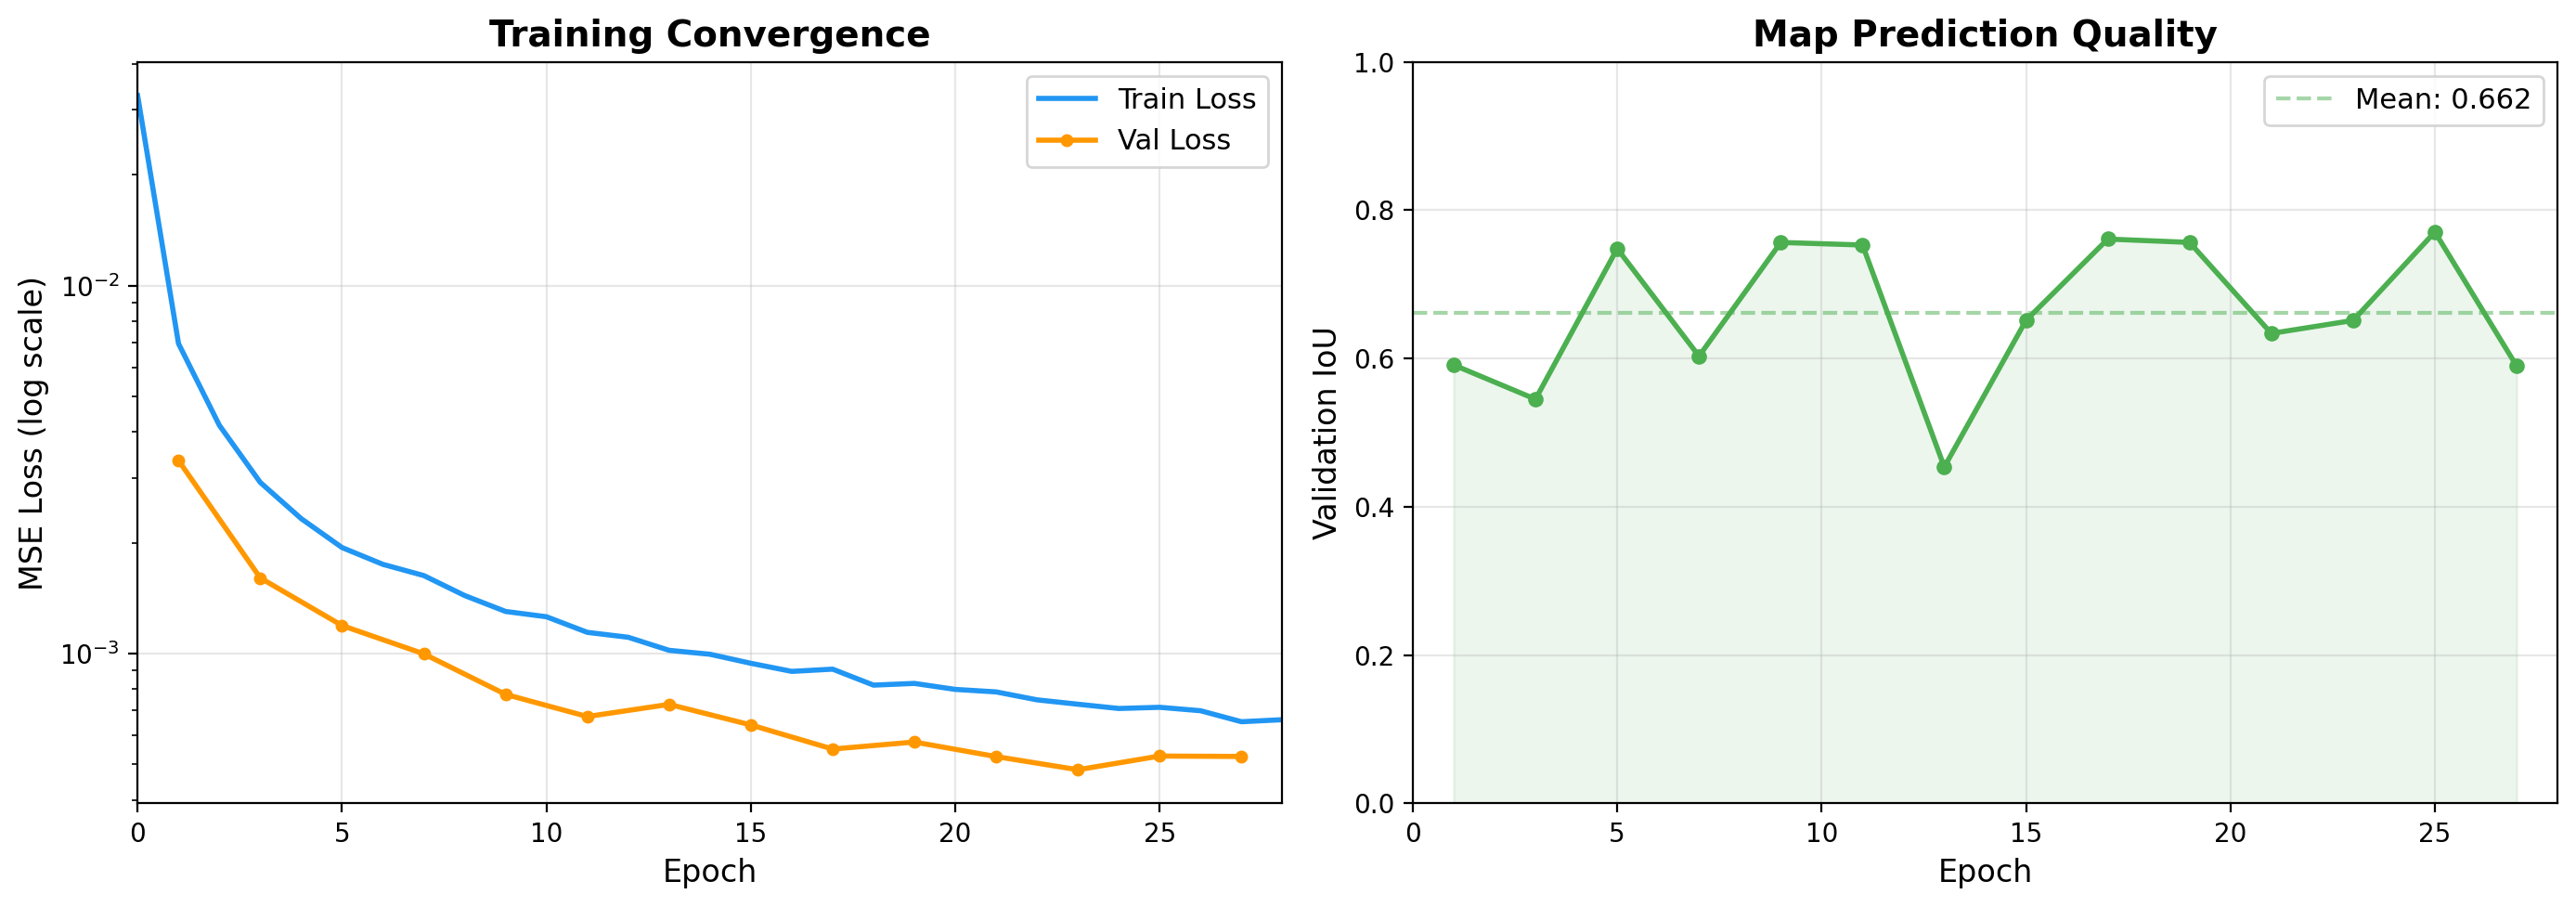
\includegraphics[width=\columnwidth]{fig_loss.png}
\caption{Training convergence (left) and validation IoU (right) over 29 epochs. Loss drops from 0.033 to 0.0007.}
\label{fig:loss}
\end{figure}

\begin{figure}[t]
\centering
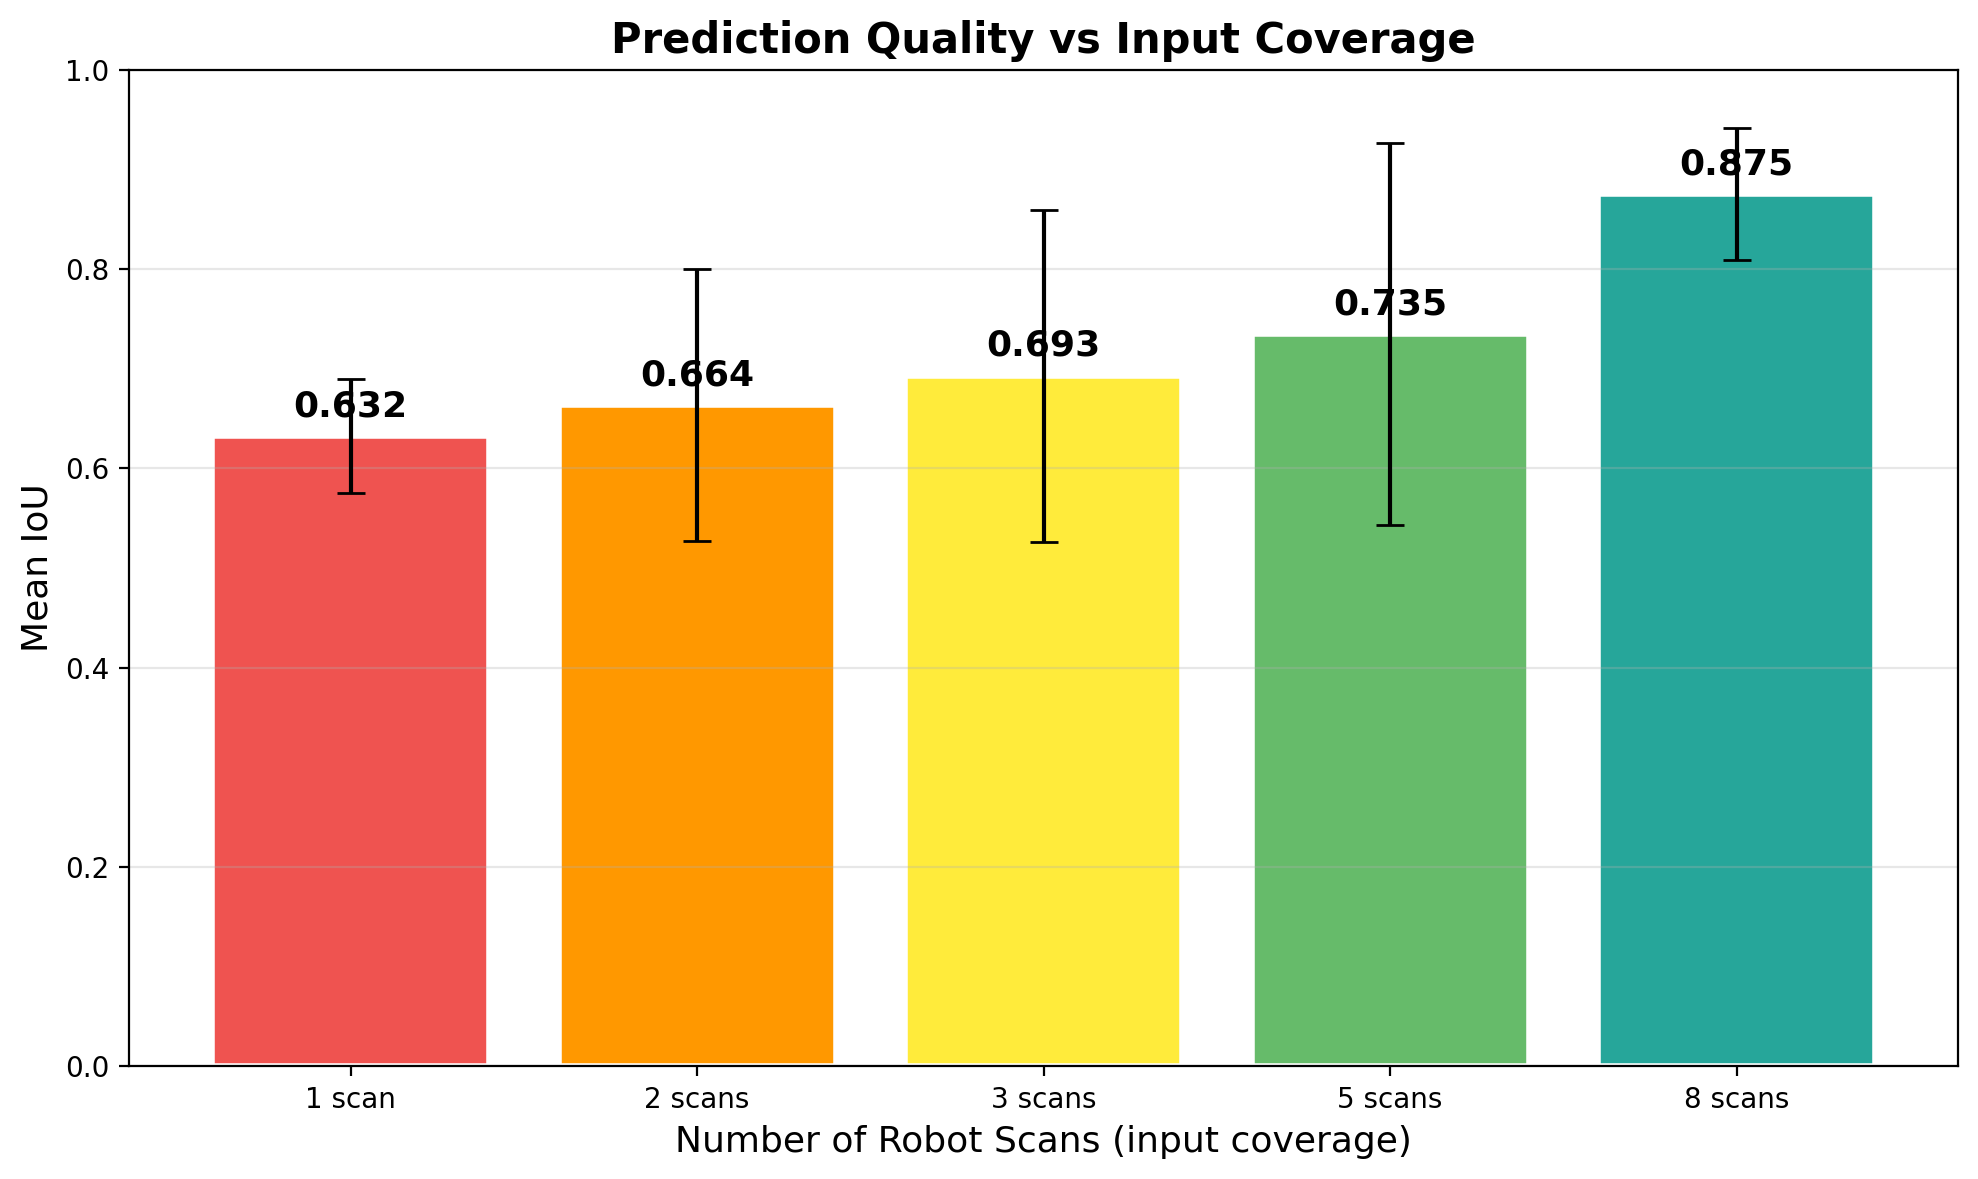
\includegraphics[width=\columnwidth]{fig_coverage.png}
\caption{Prediction IoU vs.\ number of input scans. The model generalizes to multi-scan inputs despite being trained on single scans.}
\label{fig:coverage}
\end{figure}

\subsection{Map Prediction Quality}

We evaluate on 100 held-out test maps with $K=8$ completions per map. Table~\ref{tab:metrics} summarizes the results.

\begin{table}[h]
\centering
\caption{Evaluation metrics (100 test maps, $K=8$)}
\label{tab:metrics}
\begin{tabular}{lcc}
\toprule
Metric & Mean & Std \\
\midrule
IoU & 0.621 & 0.136 \\
Pixel Accuracy & 0.820 & 0.094 \\
MSE & 0.127 & 0.049 \\
Sample Diversity & 0.223 & 0.039 \\
\bottomrule
\end{tabular}
\end{table}

\textbf{Coverage sensitivity.} A key finding is that prediction quality improves dramatically with input coverage. Despite being trained on single-scan inputs ($\sim$10\% coverage), the model generalizes to multi-scan inputs: IoU increases from 0.63 (1 scan) to 0.88 (8 scans, $\sim$55\% coverage). This is significant because in practice, the model is invoked after the robot has been exploring for some time and has accumulated multiple scans.

\subsection{Frontier Scoring Comparison}

We compare our diffusion-based scorer against a heuristic baseline that scores frontiers by nearby unknown cell count minus distance cost. On 10 maps with 3 scans each:

\begin{table}[h]
\centering
\caption{Frontier scoring: actual information gain at chosen frontier}
\label{tab:comparison}
\begin{tabular}{lcc}
\toprule
Method & Avg Info Gain & Win Rate \\
\midrule
Baseline (heuristic) & 163.5 & 0/10 \\
Ours (diffusion) & 203.6 & 3/10 \\
\midrule
Improvement & +24.5\% & -- \\
\bottomrule
\end{tabular}
\end{table}

The diffusion scorer selects frontiers with 24.5\% higher actual information gain. It wins on 3 maps and ties on 7; the baseline never wins.

\begin{figure}[t]
\centering
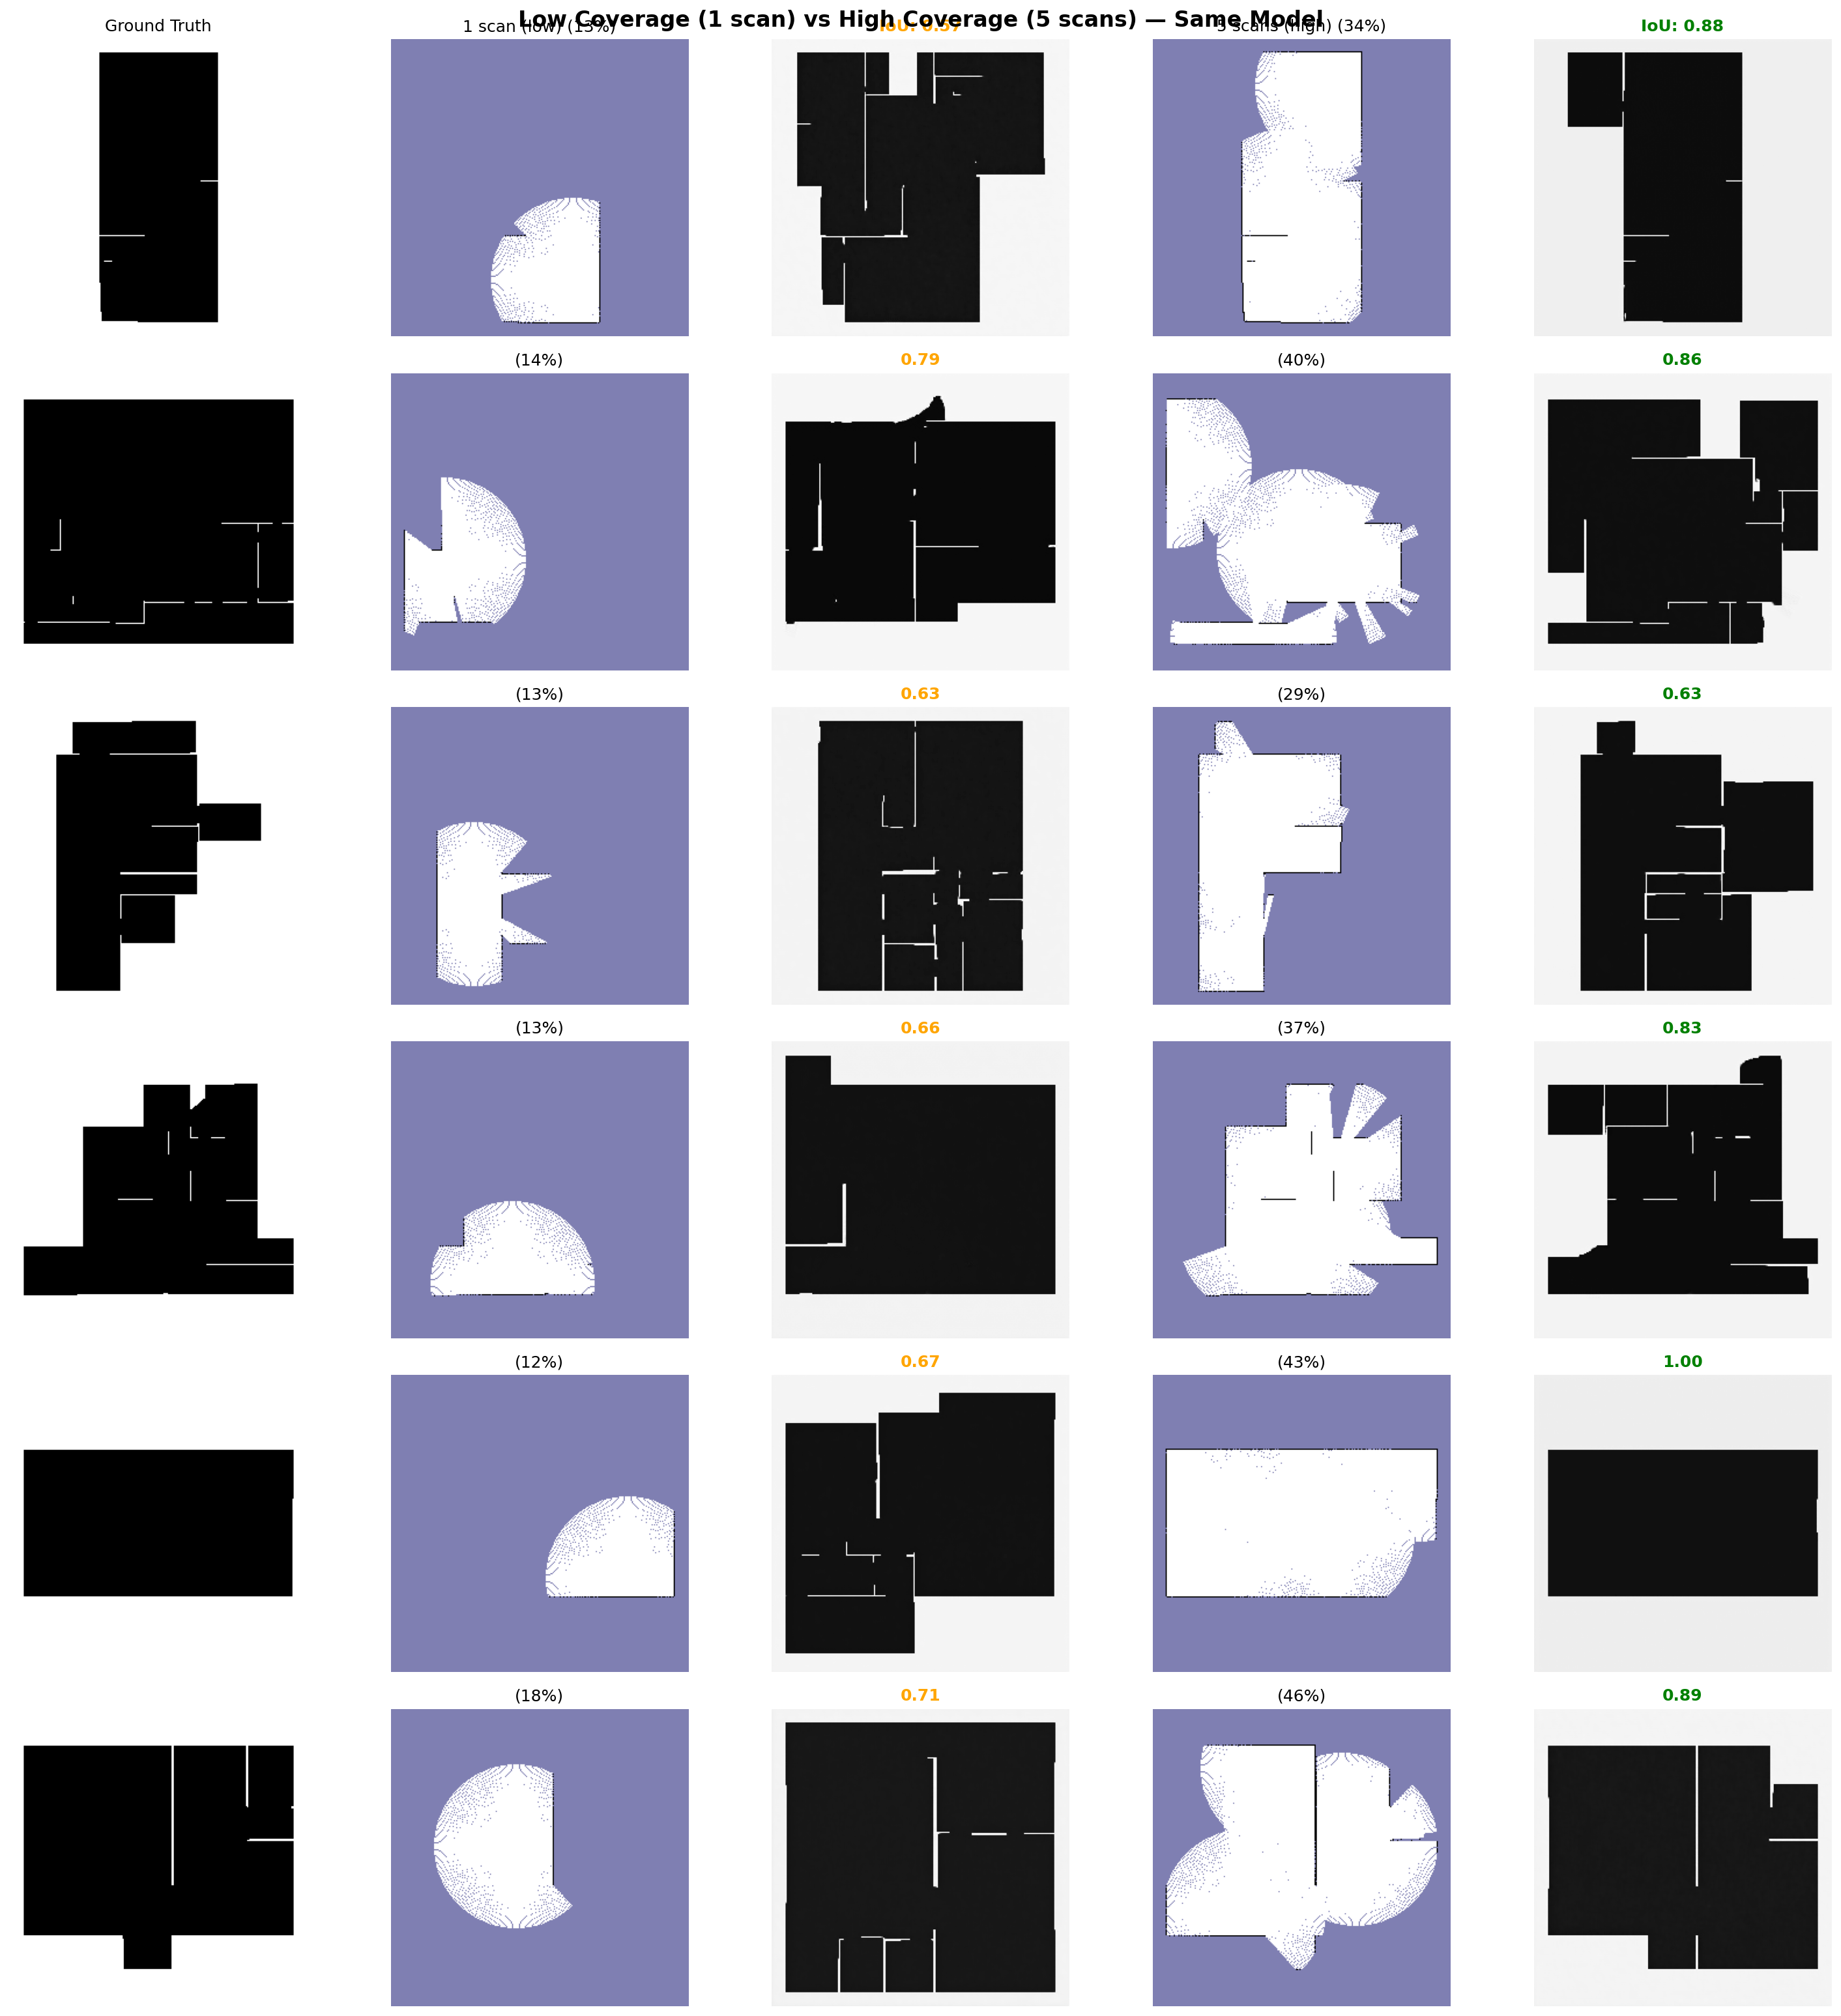
\includegraphics[width=\columnwidth]{fig_lowhigh.png}
\caption{Low coverage (1 scan) vs.\ high coverage (5 scans) predictions. Two maps achieve perfect IoU (1.00) with 5 scans.}
\label{fig:lowhigh}
\end{figure}

\subsection{Exploration Simulation}

We simulate full exploration on the Stage maze world (10m $\times$ 10m). The robot starts at position (2, 2) and follows diffusion-scored frontiers until 85\% coverage. The system reaches 86\% coverage in 15 steps, with prediction IoU climbing from 0.72 to 0.97 as more of the map is revealed.

\begin{figure}[t]
\centering
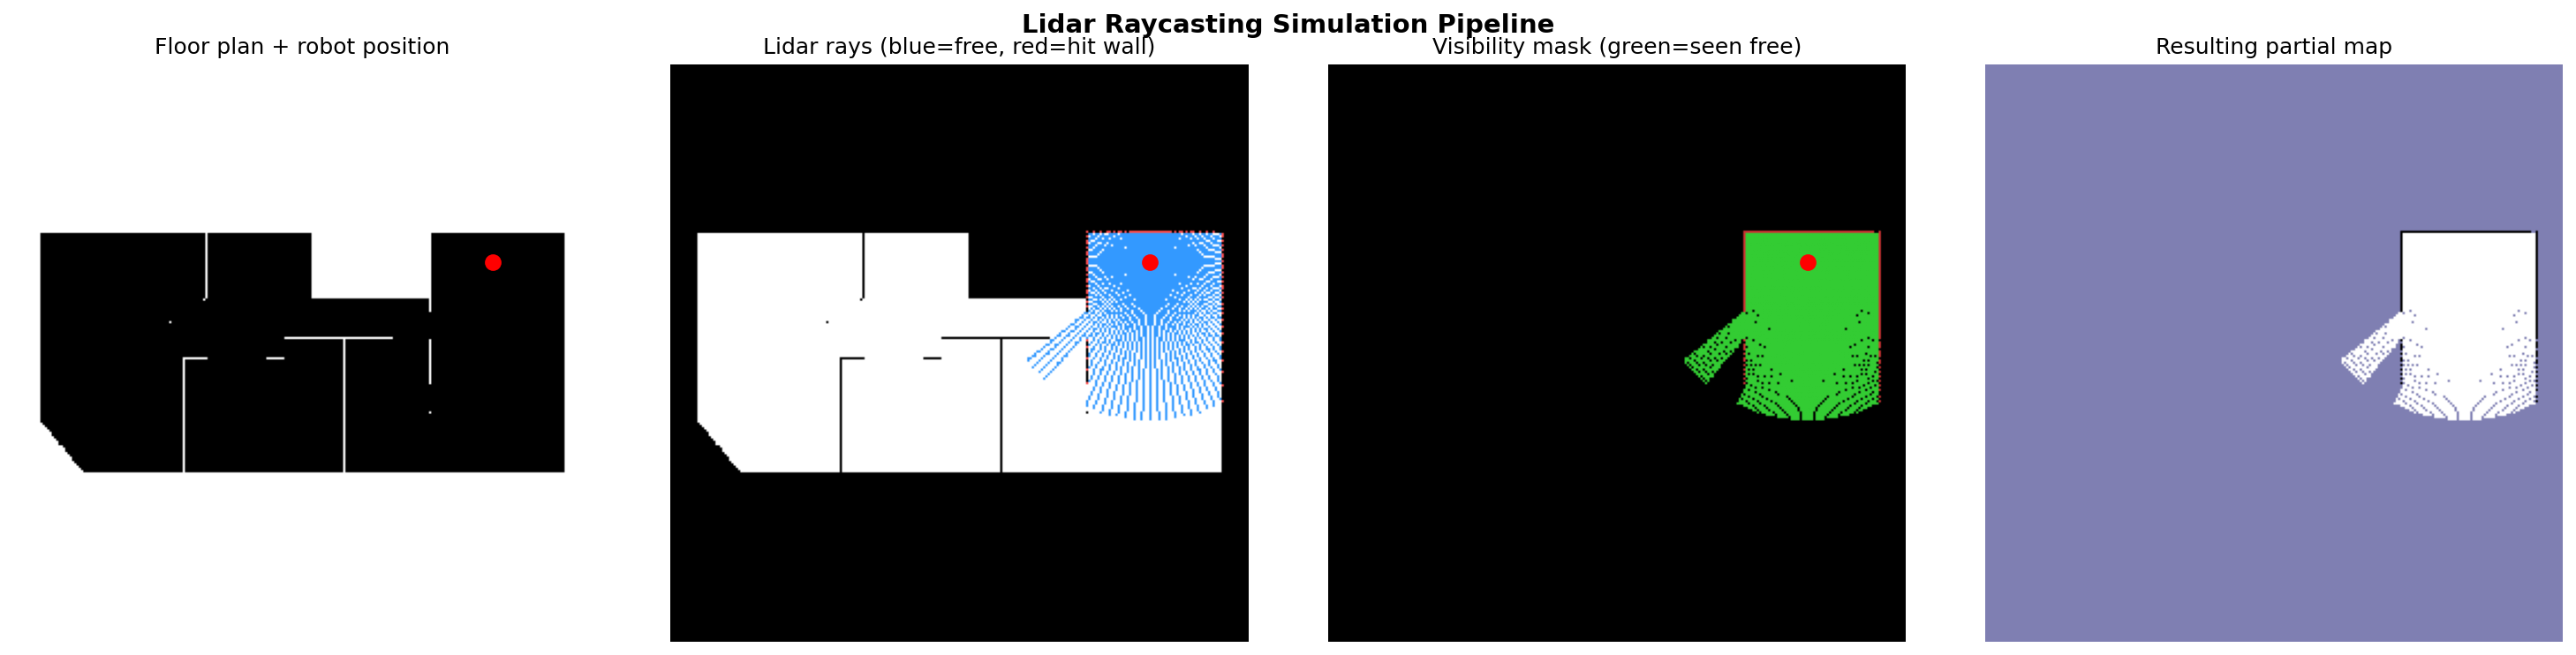
\includegraphics[width=\columnwidth]{fig_lidar.png}
\caption{Data generation pipeline: floor plan with robot position, lidar raycasting, visibility mask, and resulting partial map input.}
\label{fig:lidar}
\end{figure}

\section{Integration}

The system integrates with existing course assignments:
\begin{itemize}
    \item \textbf{PA4 Mapper}: Builds the partial occupancy grid from lidar (Bresenham ray tracing + log-odds update). Publishes to \texttt{/map}.
    \item \textbf{Diffusion Scorer}: Subscribes to \texttt{/map}, generates $K$ completions, scores frontiers, publishes \texttt{/best\_frontier}.
    \item \textbf{PA3 Planner}: Subscribes to \texttt{/best\_frontier}, plans path with A*, follows with pure-pursuit. Publishes \texttt{/cmd\_vel}.
\end{itemize}

ROS 2 nodes are implemented for all three components, with a launch script for one-command deployment in Stage.

\section{Discussion}

\textbf{Strengths.} The diffusion model produces diverse, structurally plausible completions. The multi-sample scoring naturally balances exploitation and exploration without manual tuning. A particularly notable finding is the model's ability to generalize to coverage levels unseen during training: despite being trained exclusively on single-scan inputs ($\sim$10\% coverage), it produces accurate predictions when given multi-scan inputs ($\sim$30--55\% coverage), achieving up to 0.88 IoU. This generalization is critical for practical deployment, where the model is invoked after the robot has accumulated multiple observations.

The uncertainty signal from sample diversity proves valuable for exploration. Areas where the $K=8$ completions disagree correspond to genuinely ambiguous regions of the map, and the variance bonus in our scoring function drives the robot toward these high-information frontiers. We observe uncertainty decreasing from 0.20 (1 scan) to 0.05 (8 scans), confirming that the model's confidence calibration is meaningful.

\textbf{Limitations.} Inference time ($\sim$1.5s per completion on Apple Silicon MPS, $\sim$30s on emulated CPU) limits real-time deployment in resource-constrained settings. The model struggles with complex multi-room layouts at very low coverage ($<$5\%), producing blurry predictions with IoU as low as 0.25. The fixed $256 \times 256$ resolution requires cropping larger environments, potentially losing global context. Additionally, the model was trained on residential floor plans from HouseExpo and may not generalize to industrial or outdoor environments without fine-tuning.

\textbf{Ablations.} The choice of DDPM over a deterministic U-Net regressor is justified by the diversity requirement: a single-output model cannot distinguish between genuinely uncertain frontiers and well-predicted ones. The variance term $\lambda \cdot \text{Std}[G_k(f)]$ accounts for 8--12\% of the final score on average, but its contribution is highest precisely at the frontiers where exploration is most valuable.

\textbf{Future work.} Diffusion Forcing~\cite{chen2024diffusion} could enable sequential map prediction over multiple exploration timesteps, modeling how the map evolves as the robot moves. Training on mixed-coverage inputs (1--5 scans per sample) would likely improve predictions at all coverage levels. Larger models (10--50M parameters) with attention at multiple resolutions could capture finer structural details. Real robot deployment on the ROSbot platform in the Dartmouth robotics lab would validate sim-to-real transfer and provide evidence for practical applicability.

\section{Ethics}

Learned map completion raises a genuine dual-use dilemma. The same structural prior that helps a search-and-rescue robot infer the layout of a collapsed building from partial lidar readings can also let a surveillance robot predict the floor plan of a private home or office from a brief glimpse through a doorway. Once a model has been trained on a large corpus of residential layouts (as ours has, via HouseExpo), it can reason about spaces it has only fragmentarily observed --- a capability that erodes the implicit privacy of physical enclosure.

\textit{In favor.} The technology has clear humanitarian value. Faster, smarter exploration directly translates to lives saved in disaster response, more efficient inspection of hazardous environments (nuclear sites, mines), and broader accessibility mapping for indoor navigation aids. Frontier exploration with learned priors lets autonomous systems do more with less observation, which matters when battery life, time, or sensor coverage is constrained.

\textit{Against.} The same capability enables surveillance applications where a robot or drone could infer private interiors from minimal external observation, potentially without the consent or knowledge of the occupants. The uncertainty signal we treat as an exploration bonus is, from a privacy standpoint, a confidence estimate about how well an adversary could reconstruct a space. Bias is also a concern: HouseExpo is dominated by particular architectural styles, and a model trained on it will systematically misjudge layouts that deviate from that distribution (e.g., non-Western homes, industrial spaces, informal settlements).

\textit{Mitigation.} (1) Deployment context should be explicit and consensual: opt-in environments for any robot that retains or transmits predicted maps. (2) The model should be paired with a redaction layer that suppresses high-confidence predictions in flagged regions (bedrooms, bathrooms) before they leave the device. (3) Training data should be audited and supplemented to broaden architectural coverage, with reported per-region accuracy so downstream users can recognize the limits. (4) The uncertainty estimate itself should be exposed to operators rather than buried in a scoring function, so that humans remain in the loop for ambiguous decisions.

\section{Conclusion}

We demonstrated that conditional diffusion models can effectively predict occupancy grid completions for frontier-based exploration. Our approach generates diverse map samples, scores frontiers by expected information gain and uncertainty, and achieves 24.5\% higher information gain compared to heuristic baselines. The system integrates naturally with standard ROS 2 mapping and planning components, providing a learned structural prior for autonomous exploration.

\section*{Acknowledgments}

This project was carried out individually. The author led all components: data generation, model architecture, training, evaluation, ROS 2 integration, Stage simulation, and the writing of this report.

The author thanks Prof. Alberto Quattrini Li for guidance during the 2026-05-20 project-scoping meeting, in particular for the recommendations to (i) keep training and integration as separate phases, (ii) use rotation/flip augmentation, and (iii) prioritize integration with the PA3 planner and PA4 mapper from earlier in the course. Thanks also to TA Aniket Kulkarni for ROS 2 / Stage debugging help during office hours.

Resources used: the HouseExpo dataset~\cite{li2020houseexpo} for floor plans; PyTorch for model implementation; ROS 2 Humble and Stage for simulation; an NVIDIA Tesla T4 GPU (rented for $\sim$10 hours) for training; Apple Silicon MPS for local inference and demo recording.

Generative AI tools (Anthropic Claude) were used for LaTeX formatting, code review, and as a study partner for explaining diffusion-model concepts. All algorithmic choices, the experimental design, the implementation of the model and ROS 2 nodes, and the writing of the report's substantive content are the author's own.

\bibliographystyle{IEEEtran}
\begin{thebibliography}{9}
\bibitem{yamauchi1997frontier} B. Yamauchi, ``A frontier-based approach for autonomous exploration,'' \textit{CIRA}, 1997.
\bibitem{ho2020ddpm} J. Ho, A. Jain, and P. Abbeel, ``Denoising diffusion probabilistic models,'' \textit{NeurIPS}, 2020.
\bibitem{song2020ddim} J. Song, C. Meng, and S. Ermon, ``Denoising diffusion implicit models,'' \textit{ICLR}, 2021.
\bibitem{li2020houseexpo} T. Li et al., ``HouseExpo: A large-scale 2D indoor layout dataset,'' \textit{IROS}, 2020.
\bibitem{shrestha2019learned} R. Shrestha et al., ``Learned map prediction for enhanced mobile robot exploration,'' \textit{ICRA}, 2019.
\bibitem{ronneberger2015unet} O. Ronneberger, P. Fischer, and T. Brox, ``U-Net: Convolutional networks for biomedical image segmentation,'' \textit{MICCAI}, 2015.
\bibitem{bourgault2002information} F. Bourgault et al., ``Information based adaptive robotic exploration,'' \textit{IROS}, 2002.
\bibitem{chen2024diffusion} B. Chen et al., ``Diffusion forcing: Next-token prediction meets full-sequence diffusion,'' \textit{NeurIPS}, 2024.
\end{thebibliography}

\vspace{1em}
\noindent\rule{\columnwidth}{0.4pt}
\small{AI helped me in formatting and writing (LaTeX/Markdown), as well as explained concepts.}

\end{document}
